\scanpage{114}
% archive foliation: 113
Équations explicites, en termes d'un paramètre local $t:X\longrightarrow\mathbb E^1_{\mathbb C}$, de sorte que
\[
\deleted{\unsure{*}}\quad c_0=c_{D_t}+\bar\omega_2\qquad \bar\omega_2\in\Gamma\underline\omega^2,\quad\bar\omega_2=\mu(t)\,dt^2.
\]
a) Sections horizontales $\sigma'$ de $P=\mathcal T/B$ \inserted{disjointes de $\sigma$}, correspondent aux conn. $D$ sur $\underline\omega$ telles que $c_D=c_0$, i.e. (posant $D=D_t+\underline\omega$) aux 1-formes $\underline\omega$ telles que $c_{D_t+\underline\omega}=c_0$ i.e. (puisque $c_{D_t+\underline\omega}=c_{D_t}+2D_t\underline\omega+\underline\omega^2$, $c_0=c_{D_t}+\bar\omega_2$)
\[
\Longleftrightarrow\quad 2D_t\underline\omega+\underline\omega^2=\bar\omega_2
\]
ou encore, posant $\underline\omega=\lambda(t)\,dt$
\[
(1)\qquad\boxed{2\lambda'(t)+\lambda(t)^2=\mu(t)}\qquad(\text{où }\lambda'=\tfrac d{dt}\lambda).
\]
b) Sections horizontales de $\mathcal T/B_u$, associées à $\sigma'$ section de $\mathcal T/B$ disjointe de $\sigma$. Couples $(D,\varphi)$, avec $D$ comme dessus, $\varphi\in(\Gamma\underline\omega)^*$, $D\varphi=0$. Posant $\varphi=\alpha(t)\,dt$, on aura
\[
D\varphi=D_t\varphi+\underline\omega\varphi=(\alpha'(t)+\alpha(t)\lambda(t))\,dt^2
\]
donc
\[
(2)\qquad\boxed{\alpha'(t)+\alpha(t)\lambda(t)=0}\qquad(\text{où }\alpha'\deleted{\unsure{(t)}}=\tfrac{d\alpha}{dt})
\]
\margin{i.e. $\frac{\alpha'}\alpha=-\lambda$}
i.e. $\dfrac{\alpha'(t)}{\alpha(t)}=-\lambda(t)$

ou $\log\alpha(t)=-\int\deleted{-}\lambda(t)\,dt$

ou $\alpha(t)=c\exp-\int\lambda(t)\,dt\qquad c\ c^{\mathrm{te}}\ne0$.

d) Sections horizontales de $\mathcal T$, \deleted{\unsure{une}} correspondant à une section $\sigma'$ de $\mathcal T/B$ disjointe de $\sigma$ :
\[
s:X^{\mathrm{an}}\longrightarrow\mathbb E^1(\mathbb C)\quad\text{telle que}\quad c_{D_s}=c_0
\]
i.e. $c_{D_t\deleted{\unsure{+}}-\frac{ds'}{s'}\deleted{dt}}=c_{D_t}+\bar\omega_2$

i.e. (avec 2)
\[
2D_t\left(-\frac{ds'}{s'}\right)+\left(-\frac{ds'}{s'}\right)^2=\bar\omega_2\qquad(s'=\tfrac{ds}{dt})
\]
qui s'explicite ainsi à \unsure{partir de} : $\deleted{\unsure{\frac{s''}{s'}}}-\frac{ds'}{s'}=-\frac{s''}{s'}=\lambda(t)\,dt$.

\margin{\figure{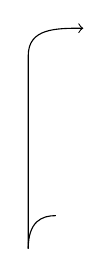
\begin{tikzpicture}[x=0.35cm,y=0.35cm]
\draw[->] (0,0) -- (0,7) .. controls (0,8) and (1,8) .. (2,8);
\draw (0,0) .. controls (0,1) and (0.5,1.2) .. (1,1.2);
\end{tikzpicture}}}
c) Sections horizontales de $\mathcal T\deleted{\unsure{B_u}}$ au-dessus de $\sigma'$ définies par $D$ ($=D_t+\underline\omega=D_t+\lambda(t)\,dt$, où $\lambda(t)$ satisfait (1), ou en satisfait à \unsure{a)}) : les $s:X^{\mathrm{an}}\longrightarrow\mathbb E^{1\mathrm{an}}_{\mathbb C}=\mathbb C$ tels que $D_s=D$, i.e. (posant $s=s(t)$) est $\frac{ds'}{s'}=-\underline\omega$ ($s'=\frac{ds}{dt}$)
\[
(3)\qquad\frac{s''}{s'}=-\lambda(t)\qquad s'=\frac{ds}{dt},\quad s''=\frac{ds'}{dt}.
\]
\unsure{On passe de c) à b)} par $\varphi=ds=s'\,dt$, i.e. $\boxed{\alpha=s'\deleted{\unsure{dt}}}$.

\[
2\left(\unsure{\frac{s''}{s'}|-\frac{s''}{s'}}\right)'+\left(-\frac{s''}{s'}\right)^2=\deleted{\unsure{\bar\omega_2}}\mu(t)
\]
i.e.
\[
-2\frac{s'''s'-s''^2}{s'^2}+\frac{s''^2}{s'^2}\ \deleted{\unsure{=}}\ \mu
\]
\[
\frac{3s''^2-2s's'''}{s'^2}=-2\frac{s'''}{s'}+3\left(\frac{s''}{s'}\right)^2.
\]
\deleted{$\unsure{\lambda'-2\lambda^2}=\mu(t)$}
\[
(4)\qquad\boxed{G_t(s)\overset{\mathrm{d\acute ef}}{=}-2\frac{s'''}{s'}+3\left(\frac{s''}{s'}\right)^2=\mu(t)}
\]
où $s'=\frac{ds}{dt}$, $s''=\frac{ds'}{dt}$, $s'''=\frac{ds''}{dt}$.

Passage de d) à c) : $s\longmapsto(\deleted{\unsure{ds}},\lambda:=-\frac{s''}{s'})$

\unsure{---} d) à b) $s\longmapsto(\alpha=s',\lambda=-\frac{s''}{s'})$

\unsure{---} d) à a) $s\longmapsto\lambda:=-\frac{s''}{s'}$.

\uline{NB} La propriété essentielle de l'expression différentielle $G_t(s)=-2\frac{s'''}{s'}+3(\frac{s''}{s'})^2$ \deleted{\unsure{est}} (\deleted{$=\frac{D_s-D_t}{dt^2}$} ($=\frac{c_{D_s}-c_{D_t}}{dt^2}$)) est son invariance par le groupe homographique :

si \deleted{$\unsure{\widetilde s=s}$}
\[
\widetilde s=\frac{as+b}{cs+d}\qquad a,b,c,d\ \text{constantes},
\]
alors $G_t(\widetilde s)=G_t(s)$ \ldots. De plus, si $\widetilde t$ est un autre uniformisant, on aura
\[
G_{\widetilde t}(s)=G_t(s)\deleted{\unsure{\cdot}}\,\widetilde t'^2.
\]

\uline{Pb} Soit $X$ courbe alg. complète sur $\mathbb C$, $t$ un uniformisant sur un ouvert $U$ de $X$, i.e. application étale $t:U\longrightarrow\mathbb E^1_{\mathbb C}$. Il existe alors une unique section $\mu$ de $\mathcal O_U$ ayant la propriété suivante : Considérons l'équation \uline{alg.} différentielle sur $U^{\mathrm{an}}$, en la fonction analytique inconnue $s:U\longrightarrow\mathbb E^1_{\mathbb C}$
\[
G_t(s)\overset{\mathrm{d\acute ef}}{=}-2\frac{\unsure{s'''|s''''}}{s'}+3\left(\frac{s''}{s'}\right)^2=\mu(t).
\]
Alors les solutions de cette équation, sur $U$
